\documentclass{article}
\usepackage{graphicx,enumerate}
\usepackage[margin=0.7in]{geometry}

\title{Ground Fault Circuit Interrupt Report}
\author{Patrick Harrington}

\begin{document}
\maketitle

\section{Introduction}

Ground Fault Circuit Interrupts (GFCI's or GFI's) are a type of protection
circuit commonly seen in bathrooms, kitchens and outdoor power sockets. Their
existence is to reduce the risk of an immediately lethal electrical shock, such as a
toaster being dropped in a bathtub full of water. Most circuit breakers are
intended to handle very large currents and trip after a relatively long
time \cite{breakrate}.A potentially lethal electric shock can
occur at very small currents as small as 30mA \cite{death}. Since
circuit breakers are slow to trip and are designed to only trip under massive
amounts of current, an extra safety measure for household plugs is essential.

\section{General Design and Theory of Operation}

GFCI's have many different names throughout the world, but they are part of a broader family of
devices known simply as \emph{Residual Current Devices}, or RCDs. These
devices detect currents in the range of 5-30mA, and can disconnect much more
quickly than a circuit breaker. 

\begin{figure}[h!]
  \centering
  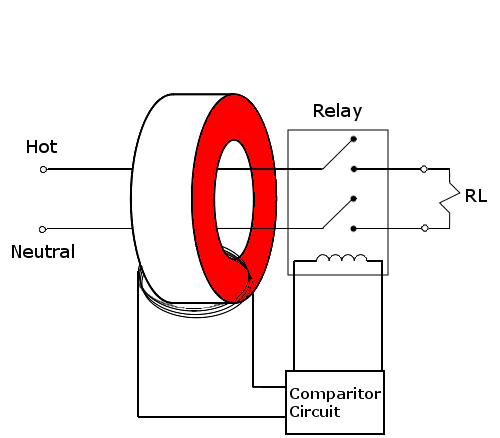
\includegraphics[scale=0.7]{circ.png}
  \caption{Circuit diagram of a GFCI}
  \label{fig:1}
\end{figure}

\newpage

The most important part of an RCD is the current transformer that measures the
difference in current through the live and neutral conductor. If the
difference is not zero, then this means there is current \emph{leaking} out of
the circuit. Control logic will then disconnect the circuit. As seen in Figure
1 below, the relay will disconnect the circuit if it detects anything unusual
from the current transformer.\cite{safety}


\begin{thebibliography}{9}

\bibitem{breakrate}
  \emph{Circuit Breaker Characteristic Trip Curves and Coordination}.
  Bulletin No. 0600DB0105,
  Cedar Rapids, IA, USA,
  August 2001.

\bibitem{death}
  Lipman, Everett A,
  \emph{Electrical Safety Information}.
  Santa Barbara, CA, USA,
  August 2007
\bibitem{safety}
  \emph{CPSC Fact Sheet, Pub. 099}.
  U.S. Consumer Product Safety Commission,
  Bethesda, MD, USA,
  Accessed April 2014
\end{thebibliography}

\end{document}
